\newif\ifsubmission
%\submissionfalse
\submissiontrue

\documentclass[12pt]{ruthesis}
\usepackage{graphicx}
\usepackage{subcaption}
\usepackage{multirow}
\usepackage{appendix}
\usepackage{url}
\usepackage{algorithm}
\usepackage{algorithmic}
\usepackage{amsmath}
\usepackage{color}
\let\labelindent\relax %to avoid conflict with IEEEtran
\usepackage{enumitem}
\usepackage{listings}
\usepackage{numprint}

\npthousandsep{,}\npthousandthpartsep{}\npdecimalsign{.}
\graphicspath{{figs/}}


\ifsubmission
  \newcommand{\TODO}[1]{}
  \newcommand{\CHANGED}[1]{#1}
\else
  \newcommand{\TODO}[1]{\textcolor{red}{TODO: #1}}
  \newcommand{\CHANGED}[1]{\textcolor{blue}{#1}}
\fi

\newcommand{\remove}[1]{}

\newcommand{\chap}[1]{Chapter~\ref{#1}}
\newcommand{\sect}[1]{Section~\ref{#1}}
\newcommand{\fig}[1]{Figure~\ref{#1}}
\newcommand{\tab}[1]{Table~\ref{#1}}
\newcommand{\alg}[1]{Algorithm~\ref{#1}}

\newcommand{\BigO}[1]{\ensuremath{\mathcal{O}\bigl(#1\bigr)}}


\title{TinyGarble: Efficient, Scalable, and Versatile Privacy-Preserving Computation Through Sequential Garbled Circuit}

\author{Ebrahim M. Songhori}
\department{Electrical and Computer Engineering}
\school{Rice University}
\degree{Doctor of Philosophy}

\committee {
Farinaz Koushanfar, Advisor \\
Professor of Electrical and Computer Engineering \\
University of California, San Diego, CA
\and
Joseph R. Cavallaro, Chair \\
Professor of Electrical and Computer Engineering and Computer Science
Rice University, Houston, TX
\and
Aydin Babakhani\\
Assistant Professor of Electrical and Computer Engineering\\
Rice University, Houston, TX
\and
Dan Wallach\\
Professor of Computer Science and of Electrical and Computer Engineering\\
Rice University, Houston, TX
\and
Ahmad-Reza Sadeghi\\
Professor Computer Science\\
Technische Universit{\"a}t Darmstadt, Darmstadt, Germany
}

\address{Houston, Texas}
\donemonth{March} \doneyear{2017} \makeindex
\begin{document}

  \begin{frontmatter}
   \pagenumbering{roman}
   %\makecover
   \maketitle
   % !TEX root = 0_main.tex
\thispagestyle{empty}
\begin{abstract}
Ever increasing demand for high data rate wireless transmissions with high spectral efficiency leads to utilization of communication systems with multiple transmit and receive antennas. In addition, excellent error-rate performance can be achieved with iterative receiver structure composed of inner detection and outer decoding. In this work we design algorithms and architectures for iterative wireless receivers with multiple antennas that are applied in both downlink and uplink scenarios. It is our goal to develop wireless receivers with implementable hardware cost, excellent error-rate performance while achieving high data rates in the order of 1 Gbps.

Soft sphere detection algorithm with reduced computational complexity based on probabilistically bounded candidate-search process is proposed. The error-rate performance are improved compare to other bounded soft sphere detection schemes for the same hardware cost. Partial candidate-search process called QRD-QLD detection is also developed for fast mobile downlink receivers. It has significantly smaller detection latency than the well-known QRD-M algorithm proposed for several emerging wireless systems. The error-rate performance are equivalent for identical hardware complexity. We apply bounded soft sphere detection in the single-carrier uplink receiver specified for the 3GPP-LTE wireless standard. By applying sphere post-detection after MMSE-based channel pre-equalization, the interference from multiple users is successfully suppressed with limited increase of computational complexity. Cost-efficient high-speed architecture design of soft sphere detector based on bounded candidate-search has been also implemented.

Outer LDPC decoding is used at the receiver back-end. Different levels of processing parallelism for outer structured semi-parallel LDPC decoders are investigated. We propose estimation methodology that quickly and accurately determines decoder architecture with the best tradeoff between area cost, decoding throughput and error-rate performance. Two decoder architectures with different levels of processing parallelism are implemented. Block-structured LDPC codes are designed for particular inner soft sphere detector and channel environment supporting modular high-speed decoder architectures. Finally, we propose methodology to estimate level of processing parallelism for the physical layer portion of iterative receiver necessary to achieve real-time data-rates of future wireless systems, such as the 1 Gbps downlink transmission.
\end{abstract}

   %% !TEX root = 0_main.tex
\chapter*{Acknowledgements}
\thispagestyle{empty}

I like to acknowledge ...

\clearpage

   \tableofcontents
   \listoffigures
   \listoftables
%   % !TEX root = 0_main.tex
\begin{dedication}
To my fianc\'ee, Zeinab.
\end{dedication}

  \end{frontmatter}
\pagenumbering{arabic}

\linespacing{1.7}

% !TEX root = 0_main.tex
\chapter{Introduction}
\label{ch:Intro}
Ever increasing demand for high data rate wireless transmissions with high spectral efficiency leads to utilization of communication systems with multiple transmit and receive antennas. Excellent quality of service represented with near-channel capacity error-rate performance can be achieved with iterative receiver structure composed of inner soft detection and outer soft-input soft-output decoding. Emerging wireless standards such as:~Wireless Local Area Network (W-LAN), Worldwide Interoperability for Microwave Access (WiMAX), $3^{rd}$ Generation Partnership Project Long Term Evolution (3GPP-LTE), etc are being constantly revised to provide higher data rates and better error-rate performance. Iterative receivers based on inner soft detection and outer decoding are promising solutions.

In this thesis, we propose to address issues of designing efficient physical layer receiver structure targeting its use in emerging wireless systems, including both downlink and uplink scenarios. It is our goal to develop performance-efficient wireless receiver with implementable hardware cost while achieving data throughputs in the order of hundreds MBits/sec.

\section{Motivation}
\label{sec:Motivation}
Excellent error-rate performance in MIMO environment are made possible by employing sophisticated algorithms such as maximum \emph{a posteriori}~(MAP) detection techniques and outer channel decoding that provides error-correction in the presence of multiple access interference, burst channel fading, channel multi-paths, additive receiver noise, etc. An approximation of impractically complex optimal joint detection/decoding is achieved by iteratively improving the \emph{a posteriori} probabilities (APPs) of transmitted coded bits between inner soft detection and outer decoding~\cite{songhori2015tinygarble}. Inner detection is typically based on the simplification of exponentially complex maximum-likelihood~(ML) approach such as the sphere detection~\cite{wang2015secure}.

% !TEX root = 0_main.tex
\chapter{Preliminaries and Background}\label{chap:prem}
In this section, we provide preliminaries and related background on garbled circuits (\chap{sec:preli_GC}) and HDL synthesis (\chap{sec:synthesis}).

\section{Background on Garbled Circuit}\label{sec:preli_GC}
Yao introduced the GC protocol for 2-party Secure Function Evaluation (SFE) in the 1980's \cite{yao1986generate}.
GC is described as a circuit whose wires carry a string valued-token instead of a bit.
Consider two parties, Alice and Bob, who want to evaluate a function $f(\cdot)$ without revealing their inputs to each other.
The function needs to be represented as a combinational Boolean circuit.
To begin with, we assume the circuit consists of a single gate with two input wires, $w_{a}$, $w_{b}$ and one output wire $w_{c}$.
Alice knows the value of input $w_{a}$ denoted by $v_{a}$ and Bob knows the value of input $w_{b}$ denoted by $v_{b}$.
The gate is also represented by a four-entry truth table $G[v_{a}, v_{b}]$.
There are two main phases in Yao's protocol.
First, Alice encodes or garbles the circuit by generating garbled tables.
Second, Bob evaluates the output denoted by $v_{c}$ without knowing anything about $v_{a}$ other than what can be deduced from the output and his own input.

The steps of Yao's approach are described below.

\begin{enumerate}
\item
	For each wire $w_a$, Alice selects one random bit $t_a$ called \emph{type} and two random $(k-1)$-bit values $Y_a^{0}$ and $Y_a^{1}$, where $k$ is a symmetric security parameter (e.g., $k=128$).
	The concatenations of the first random string and the type $X_a^{0} =  Y_a^{0}\parallel t_a$ and $X_a^{1} =  Y_a^{1}\parallel \bar{t}_a$ are called token for semantic bit $0$ and $1$ respectively.

\item
	For each gate, Alice symmetrically encrypts the respective output tokens with the four possible combinations of the input tokens.
	The resulting table of ciphertexts is called \emph{garbled table}.

\item
	Alice sends to Bob the garbled tables and the token corresponding to her input value.

\item
	Bob obliviously receives the tokens corresponding to his input through oblivious transfer (OT) \cite{rabin2005exchange}.

\item
	Bob decrypts the corresponding entry in the garbled table based on the received input tokens and gets the output token.

\item
	Finally, Alice reveals the type of the output and Bob determines its semantic value.
\end{enumerate}

In general, the circuit consists of multiple gates.
Yao's protocol for this case is described below.

\begin{enumerate}
\item
	Alice chooses tokens for all the wires, constructs the garbled tables for each gate and sends these to Bob along with the tokens corresponding to her inputs.
\item
	Bob obliviously receives the tokens corresponding to his input values through oblivious transfer.
\item
	Using these tokens, Bob evaluates the circuit gate-by-gate until he evaluates all gates.
\item
	Finally, Alice reveals the type of the outputs and Bob determines their semantic values.
\end{enumerate}

We assume the honest-but-curious model as the basis for building a stronger security protocol.
Generic ways of modifying GC-based protocols such that they achieve security against stronger malicious adversaries have been proposed, e.g., \cite{lindell2007efficient, lindell2012secure}.

In our implementation, we make use of state-of-the-art optimizations for garbled circuits as described below.

\subsection{Free XOR~\cite{kolesnikov2008improved}}
In this method, Alice generates a global random ($k-1$)-bit value $R$ which is just known to her.
During garbling operation for any wire $w_a$, she only generates a token $X_a^{0}$ and computes the other token $X_a^{1}$ as $X_a^{1} = X_a^{0} \oplus (R \parallel 1)$.
With this convention, the token for the output wire of the XOR gates with input wires $w_{a}$, $w_{b}$ and output wire $w_{c}$ can be simply computed as $X_{c} = X_{a} \oplus X_{b}$.
The proof of security for this optimization is given in \cite{kolesnikov2008improved}.

\subsection{Row Reduction~\cite{naor1999privacy}}
This optimization reduces the size of the tables for the non-XOR gates by $25\%$.
Here, instead of generating a token for the output wire of a gate randomly, the output token is produced as a function of the tokens of the inputs.
Alice generates the output token such that the first entry of the garbled table becomes all $0$ and no longer needs to be sent.

\subsection{Garbling With a Fixed-key Block Cipher~\cite{bellare2013efficient}}
This method allows to efficiently garble and evaluate non-XOR gates using fixed-key AES.
In this garbling scheme which is compatible with the Free XOR and Row Reduction techniques, the output key $X_{c}$ is encrypted with the input token $X_{a}$ and $X_{b}$ using the encryption function $E(X_a,X_b,T,X_c) = \pi(K) \oplus K \oplus X_c$, where $K=2X_a\oplus4X_b\oplus T$, $\pi$ is a fixed-key block cipher (e.g., instantiated with AES), and $T$ is a unique-per-gate number (e.g., gate identifier) called \emph{tweak}.
The proof of security is given in~\cite{bellare2013efficient}.

\section{Background on HDL Synthesis}\label{ssec:synthesis}
HDL synthesis refers to the process of translating an abstract form of  function (circuit) presentation to the gate-level logic implementation using a series of sophisticated optimizations, transformations, and mapping \cite{Techreport:Sentovich1992,Book:DeMicheli1994,Book:Devadas1994,TCAD:Brayton2006}.
An HDL synthesis tool is a computer program which typically accepts the input circuit in some algorithmic form, logic equation, or even a table, and outputs an implementation suitable for the target hardware platform.
Classic commercial/open-source HDL synthesis tools accept the input functions in the HDL format, e.g., Verilog or VHDL~\cite{tool:DesignCompiler,tool:ABC,tool:Encounter,tool:HDLdesigner,tool:PandA,tool:MyHDL} but newer ones also accept high level format, e.g., C/C++~\cite{Gupta2004, tool:Vivado}.
The common target hardware platforms for the synthesized logic include Field Programmable Gate Arrays (FPGA), Programmable Array Logic (PAL), and Application-Specific Integrated Circuits (ASIC).

The input functions (circuits), regardless of their HDL or higher level format, can be defined by the implementer to be purely combinational logic that is fully representable by Boolean functions, or they might be sequential logic which is a more general format.

Typical practical implementations of a logic function utilize a multi-level network of logic elements.
The tools translate the input to the implementation in two steps: (i) Logic minimization; and (ii) logic optimization.
Logic minimization simplifies the function by combining the separate terms into larger ones containing fewer variables.
The best known algorithm for logic minimization is the ESPRESSO algorithm~\cite{book:Brayton1984}; although the resulting minimization is not guaranteed to be the global minimum, it provides a very close approximation of the optimal, while the solution is always free from redundancy.
This algorithm has been incorporated as a standard logic function minimization step in virtually any contemporary HDL synthesis tool.

Logic optimization takes this minimized format, further processes it, and eventually maps it onto the available basic logic cells or library elements in the target technology.

Mapping is limited by factors such as the available gates (logic functions or standard cells) in the technology library, as well as the drive sizes, delay, power, and area characteristics of each gate.

Newer generations of synthesis programs, referred to as high level synthesis (HLS) tools, accept other forms of input in a higher level programming language \cite{Chapter:Zhang2008,ICCD:Chu89,TCAD:Corazao2006}, e.g., ANSI C, C++, SystemC, or Python.
HLS tools are also available in both open-source and commercial forms, cf. \cite{tool:Vivado,tool:MyHDL,tool:PandA}.
The limitation of the higher level languages is that the behavior of the function is typically decoupled from the timing.
The HLS tools handle the micro-architecture and transform the untimed or partially timed functional code into a fully timed HDL implementation, which in turn can be compiled by a classic synthesis tool.
It is well-known that the performance of the circuits resulting from automatically compiled HLS code into HDL is inferior to the performance of functions directly written in HDL.
Therefore, the main driver for the development of HLS tools is user-friendliness and not performance.

% !TEX root = 0_main.tex
\chapter{Global Flow}\label{chap:global}
The global flow of \sys{} is shown in \fig{fig:globalflow}.
It consists of the following four steps:

\begin{figure*}
\centering
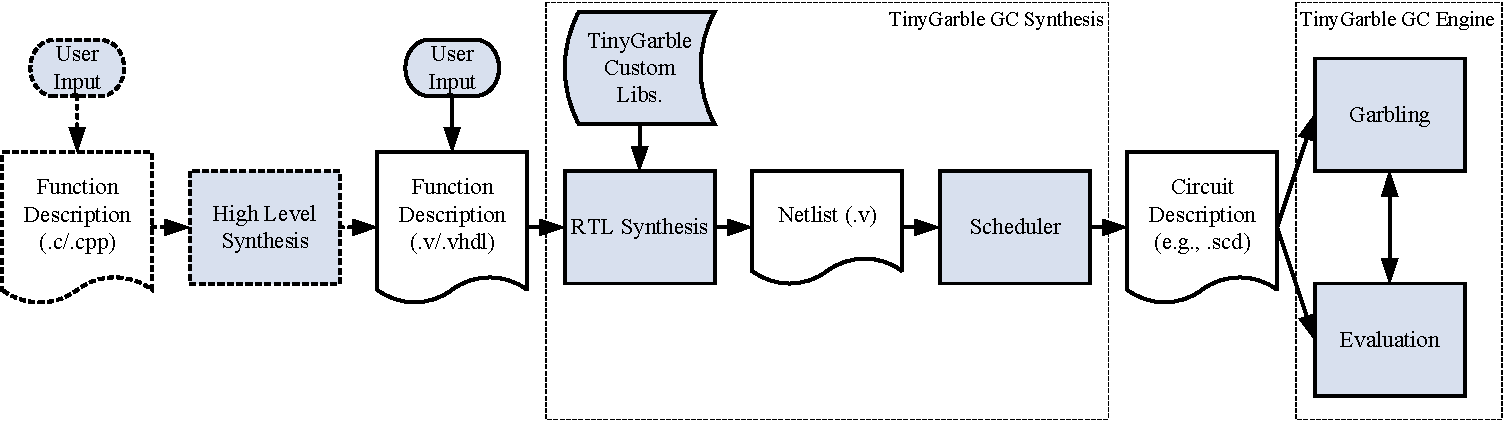
\includegraphics[width=0.95\textwidth]{flow_chart-crop.pdf}
\caption{Global flow of \sys{} for both combinational and sequential synthesis.
  The inputs can be either a C/C++ program (translatable to HDL via a standard HLS tool) or a direct HDL description.
  \sys{} is able to provide circuit description for any given GC framework.}
\label{fig:globalflow}
\end{figure*}

\begin{enumerate}
\item
  The input to the \sys{} framework is a file that describes a sequential or combinational function written in an HDL like Verilog or VHDL.
  The function can also be written in a high level language like C/C++ and automatically translated to HDL using an HLS tool.
  In the sequential circuit, the degree of folding is specified by the user.

\item
  A standard HDL synthesis tool compiles the HDL to generate a netlist file.
  The synthesis tool optimizes the netlist based on the user defined objectives/constraints and a customized library.

\item
  The netlist is parsed and topologically sorted.
  If the circuit is sequential, only its combinational part is sorted.
  Then, the sorted netlist is saved in a format compatible with any given GC framework e.g., Simple Circuit Description (SCD) compatible with JustGarble~\cite{bellare2013efficient}.

\item
  The circuit description is provided to both the garbler and evaluator to securely evaluate the function by the GC framework.
\end{enumerate}

\begin{figure*}
\centering
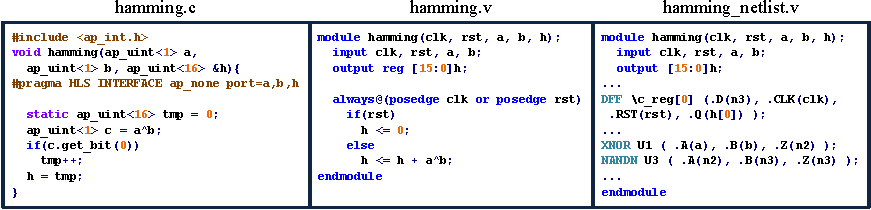
\includegraphics[width=\textwidth]{HLS_HDL_netlist-crop.pdf}
\caption{Sample files at the different steps of \sys{}'s flow for Hamming distance function.}
\label{fig:globalflow_sample}
\end{figure*}

\fig{fig:globalflow_sample} shows examples of files at different steps of \sys{}'s flow for the Hamming distance function.
The \textsl{hamming.c} file contains the description of the function in the C language.
The user inputs this function to a HLS tool to generate the corresponding description in Verilog.
The resulting Verilog file is functionally similar to the \textsl{hamming.v} file shown in the figure, but it may look more complicated and be less efficient as it is generated by an automated tool.
A user can also write the description directly in Verilog to have more control on the circuit and therefore a more efficient netlist.
The \textsl{hamming.v} file is provided to an HDL synthesis tool along with the \sys{} custom libraries to generate netlist \textsl{hamming\_netlist.v}.
The netlist describes the same function as \textsl{hamming.c} and \textsl{hamming.v} but uses the logic cells provided in the technology library.
The technology library contains 2-input-1-output logic cells to be compatible with front-end garbling tools~\cite{malkhi2004fairplay, bellare2013efficient}.

% !TEX root = 0_main.tex
\chapter{Garbling and Evaluating Sequential Circuits}\label{chap:sequen}
Sequential circuits can be used as a very compact circuit description.
In the following section we first describe the concept of sequential circuits (\sect{sec:sqcirc}) using an example and then explain the modifications required to garble/evaluate them.

\section{Sequential Circuits}\label{sec:sqcirc}

\begin{figure}[ht]
    \centering
    \begin{subfigure}[t]{0.35\textwidth}
        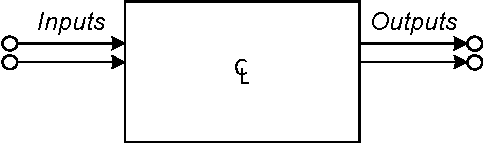
\includegraphics[width=\textwidth]{combinational-crop.pdf}
        \caption{Combinational circuit}\label{fig:combinational}
    \end{subfigure}
    \begin{subfigure}[t]{0.30\textwidth}
        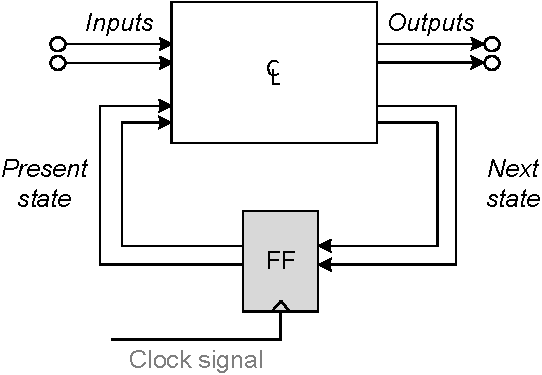
\includegraphics[width=\textwidth]{sequential-crop.pdf}
        \caption{Sequential circuit}\label{fig:sequential}
    \end{subfigure}\\
\vspace{10pt}
    \caption{(a) Combinational circuit where outputs are functions of only inputs.
(b) Sequential circuit where outputs are functions of inputs and present states.}
\end{figure}

Yao's GC algorithm allows secure evaluation of a Boolean circuit, i.e., an acyclic graph of binary gates (e.g., AND, OR, XOR, etc.).
In digital circuit theory, such a circuit is called \emph{combinational circuit} and defined as a memory-less circuit in which outputs are functions only of inputs, see \fig{fig:combinational}.

Another class of circuits in digital circuit theory are \emph{sequential circuits} in which unlike in the combinational case, circuit outputs are functions of both inputs and circuit \emph{states}.
Circuit states are kept in memory elements such as Flip Flops (FF).
The states can change at the end of each \emph{clock cycle}\footnote{The clock signal oscillates between a low and a high state and its (rising) edge is typically utilized to coordinate the memory updates.}.

As seen in \fig{fig:sequential}, a sequential circuit can be represented as an ensemble of a combinational circuit and feedback loops with memory elements.
At each clock cycle, circuit inputs as well as the present states are fed to the combinational part.
Then, it generates the outputs and next states which will be stored in the memory elements for the next cycle.
The initial value of the memory elements are either a known constant value ($0$ or $1$) or determined by an initial input value\footnote{In digital hardware, FF initialization is usually done by \emph{reset} or \emph{set} signals.
In \sys{}, we use a new signal for FF that determines the initial value.
It can be connected to a constant value or input wire.}.

\begin{figure}[h!]
    \centering
    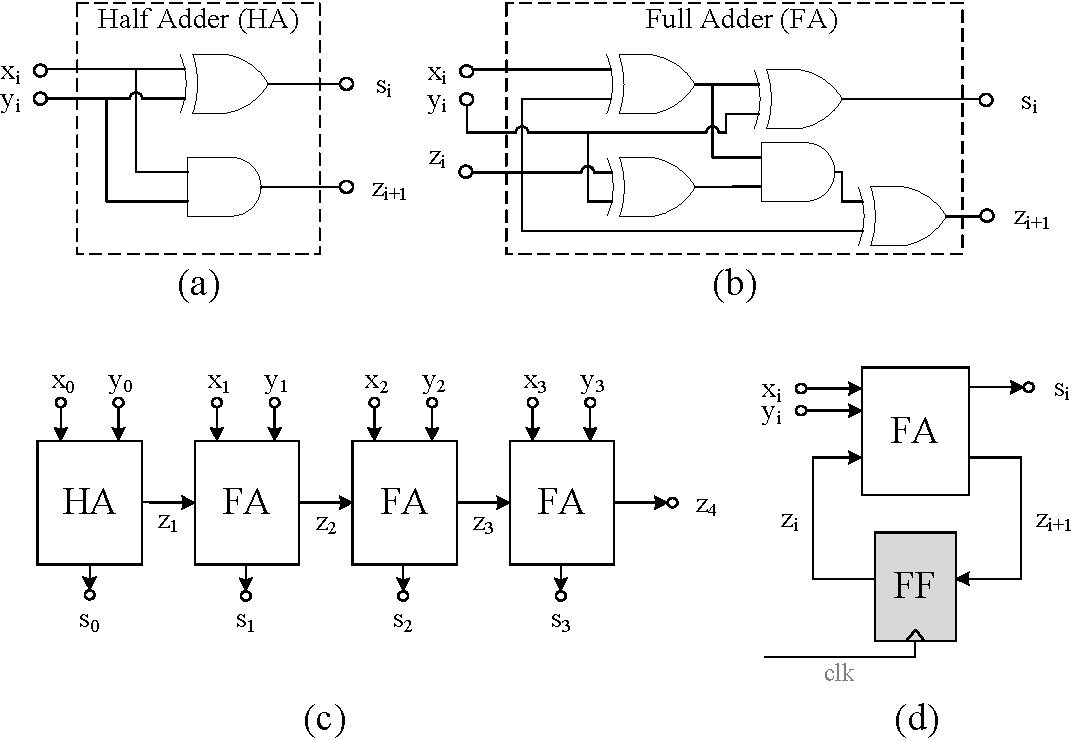
\includegraphics[width=0.7\textwidth]{adder-crop.pdf}
    \caption{Combinational and sequential design of a 4-bit Adder.
  (a) HA circuit.
  (b) FA circuit.
  (c) Combinational 4-bit Adder using 1 HA and 3 FAs.
  (d) Sequential 4-bit Adder using one FA.}\label{fig:combSeq}
\end{figure}

\fig{fig:combSeq} demonstrates an example of a combinational and a sequential implementation for a 4-bit Adder with inputs $x = \overline{x_3x_2x_1x_0}$ and $y = \overline{y_3y_2y_1y_0}$, producing sum $s = \overline{s_3s_2s_1s_0}$.
\fig{fig:combSeq}a and \ref{fig:combSeq}b show the internal combinational circuit of a half Adder (HA) and a full Adder (FA) respectively.
In \fig{fig:combSeq}c a combinational Adder is built by cascading 3 FAs and one HA.
\fig{fig:combSeq}d represents a sequential implementation of a 4-bit Adder which uses one FA and a one bit FF to save the carry bit from the previous cycle.
The circuit should be evaluated in 4 cycles.
At the first cycle the carry bit is $z_0=0$.
Note that, in the combinational circuit we use three FAs and one HA whereas in the sequential circuit, we have to use one FA for 4 sequential cycles.
This asymmetry in the loop of Addition function introduces a very small \emph{overhead} in GC computation and communication time as an HA circuit has fewer gates compared to a FA circuit.

However, the total number of gates for representing the function is reduced approximately by a factor of 4 when using a sequential circuit (one FA for sequential compared with three FA and one HA for combinational).
This helps to limit the memory footprint for garbling and evaluation required for storing circuit description and wire tokens ($k$-bit per wire, see \sect{subsec:preli_GC}).
In a sequential circuit, the number of tokens that need to be stored in memory at any moment is proportional to the number of gates in the circuit.
The wire tokens are simply over-written at each sequential cycle.
Only tokens corresponding to FFs are kept for the next cycle.

Nearly all commercial circuits used in digital hardware are designed in sequential format.
There are multiple reasons for preferring sequential circuit description over combinational including the reduction in complexity, area, power, and cost, as well as natural mapping of finite state machine control functions into a sequential format.
Some of these reasons also provide a rationale for sequential description of a function in GC, including: (i) reduction in size and memory footprint that is achieved by introducing the state elements and feedback loop from output to input; (ii) removing the need to perform costly compile-time/runtime loop unrolling by embracing loops within the sequential feedback loop; (iii) providing a new degree of freedom for folding by the placement of memory elements in the long combinational paths--the placement can be done in accordance with the user's objective.

\begin{figure}[t]
    \centering
	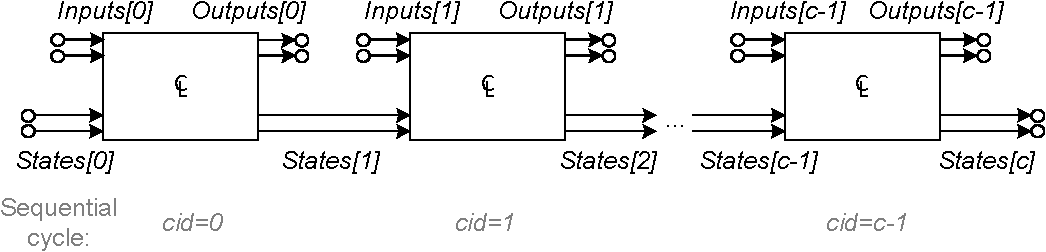
\includegraphics[width=0.8\textwidth]{sequential-open-crop.pdf}
	\caption{Functionally equivalent unrolled sequential circuit corresponding to \fig{fig:sequential}.}
	\label{fig:open-sequential}
\end{figure}

During the evaluation of a sequential circuit, the combinational block is evaluated $c$ times where $c$ is the number of sequential cycles that the circuit operates.
We can visualize this process as the unrolled combinational representation of the sequential circuit as shown in \fig{fig:open-sequential}.
The inputs/outputs of the unrolled circuit are the inputs/outputs of the combinational block in all the cycles.
The present states at each cycle $\textrm{cid}$, where $0 \le \textrm{cid} < c$, are equal to the next states at the previous cycle ($\textrm{cid}-1$).
The present states at $\textrm{cid}=0$ are equal to the input initial value.

During generation and evaluation of the garbled circuit, it must be ensured that the encryption tweaks $T$ (see \sect{subsec:preli_GC}) for each gate is unique because otherwise security is broken \cite[Sect. 3.4]{HS13}.
In \sys{}, to ensure the uniqueness property, we set tweak $T$ for each gate to be the concatenation of the cycle index (cid) and the unique gate identifiers (gid) in the combinational part of the sequential circuit, i.e., $T = \textrm{cid} || \textrm{gid}$.
\footnote{An alternative method would be to use a monotonic counter in the circuit generation/evaluation routines which is increased by one for each gate.}
As in previous work, security and correctness of the GC garbling/evaluation follow from the uniqueness of the tweak $T$ and the existing proofs of security and correctness, see \cite{LP09,bellare2013efficient}.

% !TEX root = 0_main.tex
\chapter{HDL Synthesis}\label{chap:HDL_Synth}
As described in \sect{subsec:preli_GC}, Yao's protocol requires the function to be represented as a Boolean circuit.
Previous work like FairPlay \cite{malkhi2004fairplay} and WYSTERIA \cite{rastogi2014wysteria} used custom-made languages to describe a function and generate the circuit for GC operations.
In our \sys{} framework, the user may describe a function in a standard HDL like Verilog or VHDL.
She may also write the function in a high level language like C/C++ and convert it to HDL using a HLS tool.
\sys{} uses existing HDL synthesis tools to map an HDL to a list of basic binary gates.
In digital circuit theory, this list is called a \emph{netlist}.
The netlist is generated based on various constraints and objectives such that it is functionally equivalent to the HDL/HLS input function.
Exploiting synthesis tools helps to reduce both number of non-XOR gates in the circuit and the garbling time while also making the framework easily accessible.

\section{Synthesis Flow}
In the first step, a synthesis converts functional description of a circuit into a structural representation consisting of standard logical elements.
Then, it converts this structural representation into a netlist specific to the target platform.
In both steps, the synthesis tool works under a set of user defined constraints/objectives like minimizing the total delay or limiting the area.
In the following, we describe the details of these two steps and how we manipulate the synthesis tools in each of the steps to generate optimized netlists for SFE.

\subsection{Synthesis library}
The first step in the synthesis flow is to convert arithmetic and conditional operations like add, multiply, and if-else to their logical representations that fits best to the user's constraints.
For example, the sum of two N-bit numbers can be replaced with an N-bit ripple carry adder in case of area optimization or an N-bit carry look ahead adder in case of timing optimization.
A library that consists of these various implementations is called a \emph{synthesis library}.
We develop our own synthesis library that includes implementations customized for SFE.
In this library, we build the arithmetic operations based on a full adder with one non-XOR gate \cite{BP06} and conditional operations based on a 2-to-1 multiplexer (MUX) with one non-XOR gate \cite{kolesnikov2008improved}.

\subsection{Technology library}
The next step is to map the structural representation onto a \emph{technology library} to generate the netlist.
A technology library contains basic units available in the target platform.
For example, tools targeting Field Programmable Gate Arrays (FPGAs) like Xilinx ISE or Quartus contain Look-Up Tables and Flip Flops in their technology libraries, which form the architecture of an FPGA.
On the other hand, tools targeting Application Specific Integrated Circuits (ASICs) like Synopsys DC, Cadence, and ABC, may contain a more diverse collection of elements starting from basic gates like AND, OR, etc., to more complex units like FFs.
The technology library contains logical descriptions of these units along with performance parameters like their delay and area.
The goal of the synthesis tool in this step is to generate a netlist of library components that best fit the given constraints.
For HDL synthesis, we use tools targeting ASICs as they allow more flexibility in their input technology library.
We design a custom technology library that contains 2-input gates as required by the front-end GC tools.
We set the area of XOR gates to 0 and the area of non-XOR gates to a non-0 value.
By choosing area minimization as the only optimization goal, the synthesis tool produces netlists with the minimum possible number of non-XOR gates.

An additional feature of our custom technology library is that it contains non-standard gates (other than basic gates like NOT, AND, NAND, OR, NOR, XOR, and XNOR) to increase flexibility of mapping process.
For example, the logical functions $F = A\wedge B$ and $F = (\neg A)\wedge B$ requires equal effort in garbling/evaluation.
However by using only standard gates, the second function will require two gates (a NOT gate and an AND gate) and store one extra token for $\neg A$ in the memory.
We include four such non-standard gates with an inverted input in our custom library.

For synthesis of sequential circuits, the technology library includes memory elements.
These elements can be implemented as FFs which are connected to a clock signal.
Although in conventional ASIC design FFs are typically as costly as four AND gates, in our GC application, FFs do not have any impact on the garbling/evaluation process as they require no cryptographic operations.
Therefore, we set the area of FFs to 0 to show its lack of impact on computation and communication time of garbling/evaluation.
Moreover, we modify our FFs such that they can accept an initial value.
This helps us remove extra MUXs in standard FF design for initialization.

\section{Offline Circuit Synthesis}
In \sys{}, we use HDL synthesis tools in an offline manner to generate a circuit for a given functionality.
This offline synthesis followed by a topological sort provides a ready-to-use circuit description for any GC framework.
This approach, unlike online circuit generation, does not require misspending time for circuit generation during garbling/evaluation.
It also enables the use of beneficial synthesis optimization techniques that were previously infeasible for online generation.
Moreover, the synthesis tools have a global view of the circuit, unlike previous work that manually optimized small modules of the circuit.
This allows more effective optimization for any arbitrary function and set of constraints.

However, the offline approach has certain limitations when it comes to generating circuits for extremely large functions.
Fortunately, the sequential description helps to overcome most limitations as it generates more compact circuits.
Sequential circuits are radically smaller than combinational ones with the same functionality.
This property allows synthesis tools to perform more effective circuit optimization.
Moreover, the compatibility of our sequential descriptions with standard synthesis tools simplifies the workflow of circuit generation for SFE applications.

% !TEX root = 0_main.tex
\chapter{Private Function Evaluation}\label{chap:secproc}
Two-party Private Function SFE (PF-SFE) allows secure computation of a function $f_{Alice}(\cdot)$ held by one party (Alice) operating on another party's data $x_{Bob}$ (Bob) while both the data and the function are kept private.
This is in contrast to the usual setting of SFE where the function is known by both parties.
PF-SFE is especially useful when the function is proprietary or classified.

It is well known that PF-SFE can be reduced to regular SFE by securely evaluating a Universal Circuit (UC) \cite{sander1999non}.
UC is a circuit capable of simulating any circuit (function) $f(\cdot)$ given the description of $f(\cdot)$ as input \cite{Valiant76,KS08UC}.
More formally:
$$UC(f_{Alice}(\cdot),x_{Bob}) = f_{Alice}(x_{Bob}).$$
Secure evaluation of UC completely hides the functionality of $f(\cdot)$, including its topology.
Subsequent works have shown how to allow PF-SFE while avoiding the overhead of UCs \cite{KatzM11, MohasselS13}.

A UC is similar to a Universal Turing Machine (UTM) \cite{turing1936computable,herken1995universal} that receives a Turing machine description $f_{Alice}(\cdot)$ and applies it to the input data ($x_{Bob}$) on its tape \cite{davis2001engines}.
One party provides the machine description and the other one provides the initial data.
The output $f_{Alice}(x_{Bob})$ resides on the tape after the operation is completed.
A general purpose processor is a special realization of a UTM.
It receives a list of \emph{instructions} $f_{Alice}(\cdot)$ and applies them to the input data $x_{Bob}$ in memory.

\section{Arithmetic Logic Unit}
The core of conventional processors is the Arithmetic Logic Unit (ALU) which receives two \emph{operands} and an \emph{opcode} indicating the desired operation.
ALU supports an operation set consisting of operations like addition, multiplication, XOR, etc.
The ALU circuit consists of multiple sub-circuits for these operations and a MUX which selects one of their outputs.
Secure evaluation of an ALU, where the opcode comes from one party and operands come from the other party, keeps the operations private.
Thus, ALU can be thought of as an emulator of a simple UC in which the input function $f_{Alice}(\cdot)$ is limited to a single operation.

One can combine a number of ALUs to make a more comprehensive UC that can support functions consisting of multiple operations.
Unfortunately, this approach is not practical as the complexity of the circuit grows linearly with the number of operations.
On the other hand, in conventional processors, ALUs are combined with arrays of FFs, a.k.a., \emph{registers}, in order to store the intermediate values for supporting functions with arbitrarily large number of operations.
Since none of the earlier implementations of GC explicitly supported memory elements such as FFs, the ways to connect the feedback loop around the ALU were rather limited.
However, an explicit sequential description supported by \sys{} allows us to leverage conventional processor architectures.
Therefore, the \sys{} methodology not only provides a powerful method for generating compact circuits with a low overhead for SFE, but also paves the way for systematically building scalable sequential circuits that can be used for PF-SFE.

The idea of using an ALU or a \emph{universal next-instruction circuit} in the GC protocol can also be found in \cite{liu2014automating}.
The objective of that paper was improving efficiency of SFE where the function is known by both parties, unlike PF-SFE where the function is private.
Nonetheless, instead of ALU they eventually decided to use an \emph{instruction-specific circuit} which leaks information about the function but results in less effort for non-private function evaluation.

\section{Memory}
The processor accesses the memory while executing an instruction to read the instruction and data and write the data back.
If the memory is securely evaluated along with the processor, the access patterns must be also oblivious to both parties.
On the other hand, if the memory is not evaluated securely, the access patterns could be revealed that in turn could reveal information about the function to Bob and about the data to Alice.
For example, the instruction read pattern discloses the branching decisions in the function which may leak information about the data.
Because of \sys{} sequential methodology, the memory can be easily implemented using MUX and arrays of FFs.
Thus, it can be included in the processor circuit to be evaluated securely using the GC protocol.
However, inclusion of MUXs and FFs increases the operation time and communication linearly with respect to the memory size.

One alternative approach for hiding memory access patterns is the use of Oblivious Random-Access Machine (ORAM) protocols \cite{goldreich1996software} which allows oblivious load/store operations with amortized polylogarithmic overhead \cite{gordon2012secure,liu2014automating,LO13,gentry2014garbled}.
For the sake of simplicity, we do not use ORAM in this work.
However, one can simply connect our implementation of PF-SFE to an ORAM to benefit from its lower amortized complexity.
As another alternate, \cite{ZE13} showed that algorithms can sometimes be rewritten to use data structures such as stacks, queues, or associative maps for which they give compact circuit constructions of poly-logarithmic size.

\section{Secure Processor}
We assume Alice provides the private function $f_{Alice}(\cdot)$ and Bob provides private data~$x_{Bob}$.
At the end of the operation, only Bob learns the output $f_{Alice}(x_{Bob})$.
Note that we are not considering the case where both parties learn the output as that would allow Alice to learn Bob's private data with an identity function ($f\equiv I$).
The protocol is as follows:

\begin{enumerate}
\item
  Alice and Bob agree on an instruction set architecture (ISA), its implementation (i.e., the processor circuit), the maximum number of sequential cycles, and the configuration of data $x_{Bob}$ in the memory.
\item
  Alice compiles the function $f_{Alice}(\cdot)$ according to the ISA.
  Her input is the compiled binary of the function.
\item
  Bob prepares his input based on the agreed configuration to initialize the processor memory.
\item
  Using any secure GC framework, Alice garbles the processor circuit for the maximum number of sequential cycles and Bob, after receiving his inputs with OT, evaluates the garbled processor circuit for the same number of cycles.

\item
  Alice reveals the output types such that Bob learns the value of the output $f_{Alice}(x_{Bob})$ stored in memory.
  This needs to be done only for agreed memory locations containing the outputs such that Bob does not learn intermediate values in the memory.
\end{enumerate}

Because of secure evaluation using the GC protocol in Step 4, no information about values in the circuit will be leaked except the output.
Without knowing internal values in the processor circuit, none of the parties can distinguish instructions or memory access patterns.
In the following, we demonstrate an implementation of a processor supporting the MIPS (Microprocessor without Interlocked Pipeline Stages) ISA, as an example of a garbled processor for securely evaluating private functions.

\section{MIPS}\label{sec:mips}
MIPS is a text-book Reduced Instruction Set Computing (RISC) ISA \cite{kane1992mips}.
The RISC ISA consists of a small set of simplified assembly instructions in contrast to Complex Instruction Set Computing (CISC) (e.g., x86 ISA) which includes more complex multi-step instructions \cite{hennessy2012computer}.
We choose a RISC ISA processor instead of CISC for the following main reasons: (i) lower number of non-XOR gates, (ii) simple and straightforward implementation, and (iii) availability and diversity of open-source implementations.
Moreover, we choose a single-cycle MIPS architecture (i.e., one instruction per sequential cycle).
Other architectures (i.e, multi-cycle and pipelined) increase the performance of the processor by parallelization.
However, the GC protocol does not benefit from such low level parallelization.
The only important factor for GC is the total number of non-XORs which is smaller in the single-cycle MIPS.
We follow the Harvard Architecture which has distinct instruction memory (IM) and data memory (DM) in order to separate the parties' inputs.
IM is a Read-Only Memory (ROM) that stores Alice's instructions.
DM is a Random Access Memory (RAM) that is initialized with Bob's input.
The parties' inputs are connected to the initial signal inputs of FFs in the memories.
Bob's outputs are connected to the outputs of FFs in the specified address of DM.
The output address in DM is part of the agreed memory configuration.

\begin{figure*}[t!]
\centering
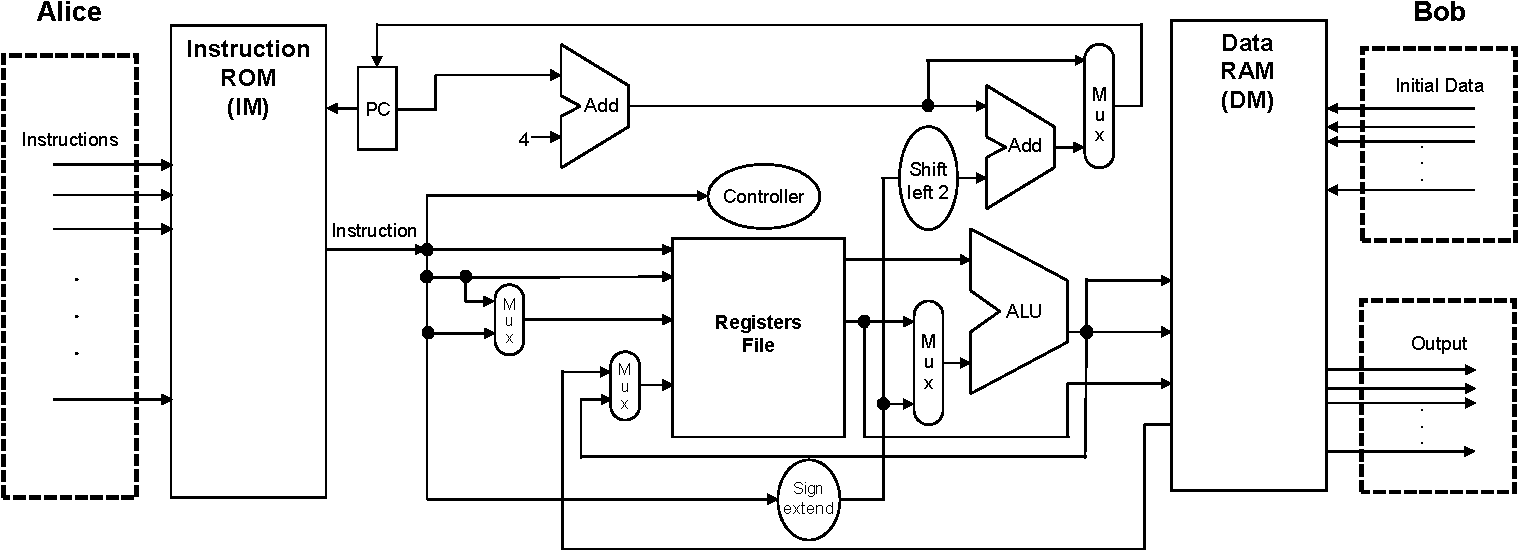
\includegraphics[width=0.95\textwidth]{mips-complex-crop.pdf}
\caption{Lite MIPS architecture.
  Alice's and Bob's inputs and the output are shown.}\label{figure:mips}
\end{figure*}

\fig{figure:mips} shows the overall architecture of our 32-bit MIPS processor.
It is based on the Plasma project in opencores \cite{rhoads2006plasma}.
We modified the circuit such that the instruction ROM (IM) and the data RAM (DM) are separated.
The original Plasma processor supports all the MIPS~I ISA except unaligned memory access.
In our implementation, we also omit division instructions because of their large overhead.
Any arbitrary C/C++ function can be easily compiled to MIPS~I assembly code using a cross-platform compiler e.g., GNU gcc.

In 32-bit MIPS, the program counter (\emph{PC}) is a 32-bit register (array of FFs) that points to the instruction being executed at the current cycle.
The instruction is fetched from IM based on the current PC value.
The \emph{controller} unit is responsible for setting signals to perform the instruction.
In 32-bit MIPS, the \emph{register file} consists of 32 registers of 32-bit each.
In each cycle, at most two registers can be read and at most one register can be written back.
ALU receives the read register(s) or a sign extended \emph{immediate} as operands.
ALU also receives an opcode from the controller unit.
The output of ALU will be either written back to the register file or fed to DM as an address for load/store.
The loaded data from DM is written back to the register file.
In each cycle, PC is incremented by 4 to point to the next instruction in IM or is changed according to a branch or jump instruction.

% !TEX root = 0_main.tex
\chapter{Evaluation}\label{chap:eval}
We use a variety of benchmark functions to evaluate the performance and practicability of \sys{}.
In this section, we first describe our experimental setup (\sect{sect:exp}) and metrics for quantifying the performance of \sys{} (\sect{ssec:metrics}).
We outline the performance comparison of \sys{} (with HDL synthesizer and our custom libraries) on combinational benchmark functions with PCF \cite{kreuter2013pcf}, one of the best known earlier automated methodologies to generate circuits for garbling in \sect{ssec:customlib}.
\sys{}'s performance in generating sequential circuits for benchmark functions using a standard HDL synthesis tool is demonstrated in \sect{ssec:seqeval}.
\sect{ssec:cacheTime} shows the CPU time for various numbers of sequential cycles which demonstrates the effect of memory footprint reduction in garbling time.
\sect{ssec:HLSeval} shows a comparison between \sys{}'s performance using an HLS tool (input written in C) and using a conventional HDL synthesis tool (input given in Verilog).
Lastly, \sect{ssec:mipsres} shows the result of our garbled processor and implementation of Hamming distance as a benchmark.

We also compare the performance of the commercial logic synthesis tool with the academic, open-source tools in Appendix \ref{app:seqos}.
We show that in most cases, the performance of the open-source tool is comparable to the commercial tool.

\section{Experimental Setup}\label{sec:setup}
The circuit generations are all done on a system with Linux RedHat Server 5.6, 8~GB of memory, and Intel Xeon X5450 CPU @ 3~GHz.
We use another system with Ubuntu 14.10 Desktop, 12.0~GB of memory, and Intel Core i7-2600 CPU @ 3.4GHz to assess the timing performance of the sequential garbling scheme in \sect{ssec:cacheTime}.

Two sets of HDL synthesis tool chains are used in our experiments: one commercial and one open-source (Appendix \ref{app:seqos}).
Our commercial HDL level synthesis tool is Synopsis Design Compiler (DC) 2010.03-SP4 \cite{tool:DesignCompiler}.
We also use the Synopsis Library Compiler from the DC package to interpret our custom technology library.
In \sect{ssec:HLSeval}, we utilize Xilinx Vivado HLS \cite{tool:Vivado}, a commercially available HLS tool whose inputs are written in the C/C++ programming language.
We emphasize that \sys{} can operate with any commercial or open-source sequential HDL-level (or HLS) synthesizer, as long as the synthesizer is capable of performing state-of-the-art logic optimization and mapping algorithms.

\section{Performance Metrics}\label{sec:metrics}
We use the following metrics to measure the efficiency of \sys{} for generating garbled circuits:

\begin{itemize}
\item
	\textit{Memory Footprint Efficiency} ($\mathit{MFE}$): $$\mathit{MFE} = \dfrac{q_{0}}{q},$$ where $q_{0}$ is the total number of gates in the reference circuit and $q$ is the total number of gates in the circuit under evaluation.
	The maximum number of tokens that need to be stored at any point during garbling/evaluation as well as memory required for storing circuit description is directly proportional to the number of gates in both sequential and combinational circuits.
	Thus, the total number of gates is approximately proportional to the memory footprint.

\item
	\textit{Number of Garbled Tables} ($\mathit{\#GT}$): $$\mathit{\#GT} = \#nonXOR\times c,$$ where $\#nonXOR$ is the number of non-XOR gates in a circuit and $c$ is the number of sequential cycles that the circuit needs to be garbled/evaluated.
	In free XOR-based GC schemes, each non-XOR gate requires a garbled table to be generated by the garbler and sent to the evaluator at each sequential cycle.
	Thus, this metric is an estimate of both the computation and communication time.

\item
	\textit{Garbled Tables Difference} ($\mathit{GTD}$ (\%)): $$\mathit{GTD} = \dfrac{\mathit{\#GT} - \mathit{\#GT}_{0}}{\mathit{\#GT}_{0}} \times 100,$$ where $\mathit{\#GT}_{0}$ is the total number of garbled tables for the reference circuit and $\mathit{\#GT}$ is the total number of garbled tables for the circuit under evaluation.
	When comparing a sequential with a combination circuit, positive $\mathit{GTD}$ shows an \emph{overhead} (caused by folding a circuit with an asymmetric loop, see \sect{sec:sequen}) in total computation and communication time resulting from an excessive number of garbled tables generated in the sequential circuits.
	However, in general, negative $\mathit{GTD}$ shows improvement in the number of non-XOR gates and generated garbled tables that results from logic synthesis optimization.
\end{itemize}

\section{Benchmark functions}\label{sec:funcs}
We evaluate \sys{}'s circuit generation method on various benchmark functions.
Several of these functions have been used in previous works, e.g., PCF~\cite{kreuter2013pcf}.
In the following, we introduce our benchmarks and explain how we fold them into a sequential representation.

\textit{Sum.} This function receives two $N$-bit inputs and outputs an $N$-bit sum.
The sum function is implemented in $N$ steps of one bit sums by keeping the carry bit.
Thus, it can be folded up to $N$ times without any significant overhead in number of garbled tables ($\mathit{\#GT}$).

\textit{Hamming Distance.} This function receives two $N$-bit inputs and outputs the $\log_2(N)$-bit Hamming distance between them.
The Hamming distance between two numbers is the number of positions at which the corresponding bits are different.
A possible combinational implementation of the $N$-bit Hamming distance uses a binary tree of adders that sums all $1$-bit values from the bit differences to a final Hamming distance consisting of $\log_2(N)$ bits \cite{BP06}.
This implementation cannot be folded easily.
However, we can fold this function into $N$-cycles of one XOR and one $\log_2(N)$-bit adder.
This causes an overhead compared to the combinational circuit.

\textit{Compare (Millionaires problem).} This function receives two $N$-bit unsigned input values and outputs a greater than signal consisting of one bit that indicates if the first input is greater than the second one.
The comparison function can be implemented in $N$ steps of subtraction by keeping the carry bit \cite{KSS09}.
Thus, it can be folded up to $N$ times without any significant overhead.

\textit{Multiplication.} This function receives two unsigned $N$-bit inputs and outputs their unsigned $N$-bit product.
The multiplication function consists of $N$ additions and shifts.
The shift operations result in an asymmetric structure in this function.
Thus, folding it up to $N$ times may increase the overhead.

\textit{Matrix Multiplication.} This function receives two $N\times N$ matrices consisting of $32$-bit unsigned numbers and outputs an $N\times N$ matrix equal to the product of the input matrices.
The $N\times N$ matrix multiplication function consists of three $N$-cycle nested loops with a symmetric structures.
It can be folded up to $N^3$ times without any significant overhead.

\textit{AES-128.} This function receives a 128-bit plaintext and 128-bit round keys and outputs a 128-bit ciphertext based on the Rijndael algorithm.
The AES-128 function consists of 10 rounds with almost symmetric structure.
Ideally, it can be folded up to $10$ times without any significant overhead.

\textit{SHA3.} This function receives $576$-bit inputs and outputs a $1600$-bit number equal to the SHA3 hash of the input.
We implement the Keccak-f permutations[$1600$] procedure for realizing this function.
The SHA3 function consists of 24 steps, each with a symmetric structure.
It can be folded 24 times without any significant overhead.

\section{Combinational Garbled Circuit}\label{sec:customlib}
To show the performance gain of using our custom libraries, we compare \sys{} combinational circuits with circuits reported in PCF \cite{kreuter2013pcf}.
We choose PCF because among the \emph{automated} GC tools available at the time of writing, it shows better results for most of the benchmarks.
In some other work like FastGC \cite{huang2011faster}, a number of benchmark circuits have been more aggressively improved (compared to PCF) using ad-hoc and mostly manual optimizations, but without a generalizable methodology.

The comparison is shown in \tab{table:result-comb}.
We compute the garbled tables difference $\mathit{GTD}$ (see \sect{ssec:metrics}) of various benchmarks by using circuits reported in PCF as reference ($\mathit{GTD}$\textsuperscript{PCF}).
It can be seen that the combinational circuits generated by \sys{} have non-positive $\mathit{GTD}$\textsuperscript{PCF} which means that the number of garbled tables are less than or equal to that of PCF circuits.
We also compare the memory footprint by computing the memory footprint efficiency $\mathit{MFE}$ with PCF as reference ($\mathit{MFE}$\textsuperscript{PCF}).
We observe that $\mathit{MFE}$\textsuperscript{PCF} is larger than 1 (up to 9.3).
This means that even without using sequential circuits, the memory footprint can be reduced by almost an order of magnitude by using \sys{} custom libraries and standard HDL synthesis.

In case of Hamming distance, \sys{} shows, on average, $80\%$ improvement in number of garbled tables.
Another automated tool CBMC-GC \cite{franz2014cbmc} reports better result compared to PCF for Hamming 160 (non-XOR $\numprint{4738}$, total gates $\numprint{20356}$).
However, \sys{} shows $66\%$ improvement in number of garbled tables compared to CBMC-GC.
In case of 256-bit and 1024-bit Multiplication, and $8\times 8$ and $16\times 16$ Matrix Multiplication, because of the huge (impractical) sizes, Synopsis DC was unable to generate the entire combinational circuit.
This is because Synopsis DC is a tool developed for commercial applications.
The real-life applications are almost always written sequentially, otherwise the design would not be scalable or even amenable to offline compilation onto a hardware circuit.
We emphasize that our sequential circuit ($c>1$) provides the exact same functionality while having a very small memory footprint compared with the reference circuit.

\subsection{Comparison with Hand-Optimized Circuits}
The netlists generated by the automated flow of \sys{} show similar performance as the hand-optimized netlists in many cases.
For example, \cite{KSS09} describe an $N$-bit sum circuit with $5N$ gates of which $N$ gates are non-XOR and an $N$-bit comparison circuit with $4N$ gates of which $N$ gates are non-XOR.
The circuits generated by \sys{} have about the same number of gates for these two functions.
Note that one can always add any hand-optimized module to the synthesis library of \sys{}.

\section{Sequential Garbled Circuit} \label{sec:seqeval}
As described in \sect{sec:sequen}, the user has the degree of freedom to fold a combinational circuit and convert it to a sequential one to reduce the memory footprint.
$c$ denotes the number of sequential cycles required to garble/evaluate the circuit.
This value demonstrates the amount of folding that is performed before the circuit is input to the synthesizer.
The user defines the value of $c$ and writes her own input function in an HDL or a higher level language such that the function is evaluated in $c$ sequential cycles.

We use Memory Footprint Efficiency ($\mathit{MFE}$), to evaluate the reduction in memory requirement.
We use \sys{} combinational circuits ($c=1$) as reference.
The ideal $\mathit{MFE}$ for a circuit with $c$ sequential cycles is $c$.
We also compare the memory footprints of sequential circuits with combinational circuits reported in PCF ($\mathit{MFE}$\textsuperscript{PCF}).

As explained in \sect{ssec:sqcirc}, the folding process may introduce some overhead on the total number of garbled tables.
To assess this overhead, we compute the Garbled Tables Difference ($\mathit{GTD}$) of the sequential circuit using \sys{} combinational circuits as reference.
The ideal $\mathit{GTD}$ is $0\%$, which means that the total number of garbled tables should be equal to those for a functionally equivalent combinational circuit.
We also compare the number of garbled tables of sequential circuits with combinational circuits reported in PCF ($\mathit{GTD}$\textsuperscript{PCF}) to show that even with the incurred overhead, the number of garbled tables for sequential circuits is still less than that of PCF for most cases.

\begin{table*}
\centering
\caption{Comparison of \sys{} combinational circuits with PCF.
In case of AES 128, the result is compared with FastGC.}
\label{table:result-comb}
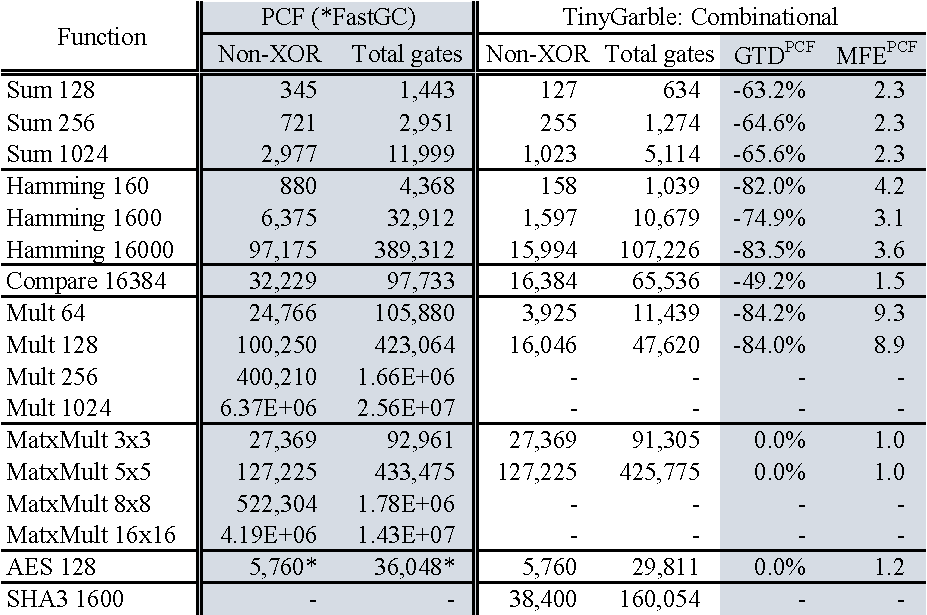
\includegraphics[scale=0.9]{results-comb-crop.pdf}
\end{table*}

\begin{table*}
\centering
\caption{Comparison of \sys{} sequential circuits with PCF and \sys{} combinational circuits.
In case of AES 128, the result is compared with FastGC.}
\label{table:result-seq}
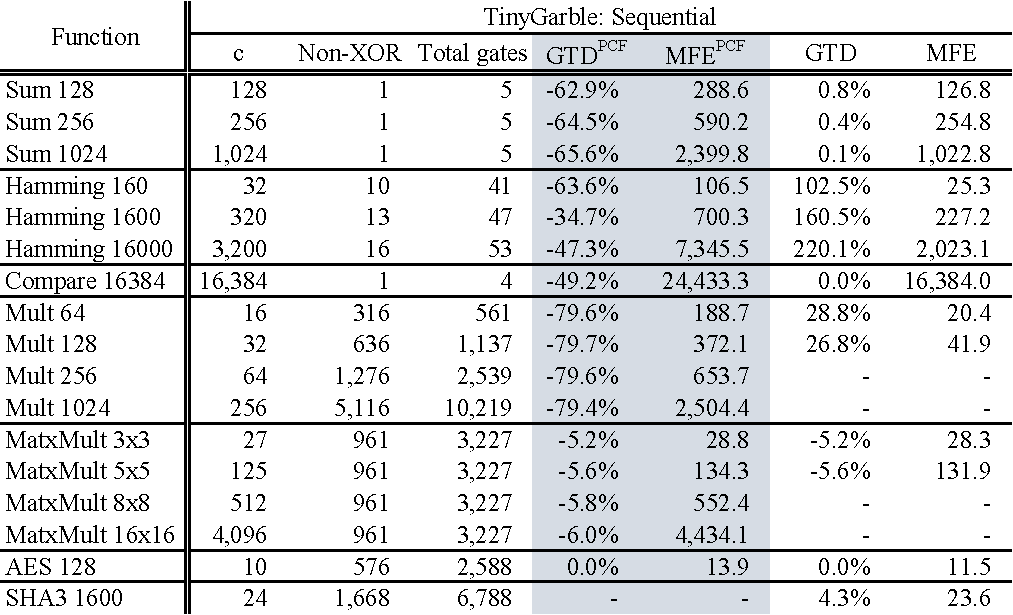
\includegraphics[scale=.9]{results-seq-crop.pdf}
\end{table*}

\tab{table:result-seq} shows the number of total gates, non-XOR gates, $\mathit{MFE}$, $\mathit{GTD}$, $\mathit{MFE}$\textsuperscript{PCF}, and $\mathit{GTD}$\textsuperscript{PCF} of the benchmark circuits for various input widths.
$\mathit{MFE}$, $\mathit{GTD}$ are computed with \sys{} combinational circuits (with $c=1$) as reference.
$\mathit{MFE}$\textsuperscript{PCF}, and $\mathit{GTD}$\textsuperscript{PCF} use the circuits reported in PCF as reference.
In the case of AES 128, we compare our implementation with the manually optimized circuit reported in FastGC \cite{huang2011faster} because PCF did not report it directly.

We provide a few highlights from \tab{table:result-seq}.
\sys{} is able to decrease the size of the sum of two $1024$-bit numbers by $\numprint{1022.8}$ times (i.e., more than three orders of magnitude) without affecting the number of garbled tables ($\mathit{GTD}$) compared with its own combinational circuit.
For Hamming 16000, \sys{} is able to decrease the memory footprint by $\numprint{7345.5}$ times (i.e., about 4 orders of magnitude) while reducing the number of garbled tables by $47.3\%$ in comparison with the circuit reported in PCF.
In case of Mult 1024, \sys{} shrinks the memory footprint by a factor of $\numprint{2504.4}$ while reducing the number of garbled tables by $79.4\%$ when compared with the result in PCF.
For a $16\times 16$ matrix multiplication, a $\numprint{4434.1}$ more compact \sys{} solution with $6\%$ less garbled tables compared with PCF is available.
By folding AES-128 10 times, the total number of gates is reduce by a factor of $13.9$ compared to the  FastGC circuit without any overhead in the number of non-XORs.
Observe that the savings are typically more for larger bit-widths while extreme foldings can introduce an increased overhead in number of garbled tables due to the resulting asymmetry.

Because of the \sys{} superior scalability, we are able to implement functions that have never been reported before, such as SHA-3, which can be represented using $\numprint{344059}$ and $\numprint{6788}$ gates respectively.

\section{Effect of Folding on Garbling Time}\label{sec:cacheTime}
So far, we have only reported the overhead in terms of garbled tables ($\mathit{GTD}$) that is a function of the number of non-XOR gates.
As explained in \cite{bellare2013efficient}, if we see garbling as a cryptographic primitive, its computation time (without considering communication) will also be interesting.
In practice, smaller circuits which can fit entirely in the processor cache result in fewer cache misses and therefore, consume less CPU cycles for garbling.
To better observe the impact of cache speed-up for the compact circuits resulting from \sys{}, \fig{fig:cpu_time} depicts the CPU Time (left y-axis) and the memory footprint of wire tokens (right y-axis) versus $c$ (x-axis) for the $\numprint{32768}$-bit Sum function.
As mentioned earlier, the memory footprint is directly proportional to the total number of gates in the sequential circuit.

This experiment is done using our sequential garbling scheme based on JustGarble \cite{bellare2013efficient} that includes using Free XOR, Row Reduction, and Fixed-key AES garbling techniques (see \sect{subsec:preli_GC}).
We use an Intel Core i7 CPU @ 3.40GHz which supports the AES-NI instruction set.
The CPU cycle is measured as the average of $10,000$ trials using RDTSC instruction.
For security parameter $k=128$ (the bit-width of wire token, see \sect{subsec:preli_GC}), we store $128$-bit per tokens.
For garbling in JustGarble, we store 2 tokens, 2 32-bit input indexes, and an 8-bit gate-type per gate.
Thus, the memory footprint is approximately $328$-bit per gate in garbling operation.
Folding the circuit by a factor of $c \in [1:\numprint{32768}]$ constantly decreases the memory footprint while the computation effort remains almost constant.
Interestingly, as can be seen from the figure, the number of CPU cycles sharply decreases by $1.6\times$ just when we fold four times ($c=4$) compared to $c=1$.
This is because for $c \geq 4$, the memory space required for garbling completely fits in the cache.
The minimum CPU cycle per gate happens at $c=\numprint{2048}$ for $3.2$~KB memory footprint.
This signifies the fact that even for large functions, we can use the sequential approach to fit the corresponding memory space requirement into the cache and avoid the penalty of cache misses, thus achieving a large reduction in garbling time.

\begin{figure}[ht]
	\centering
	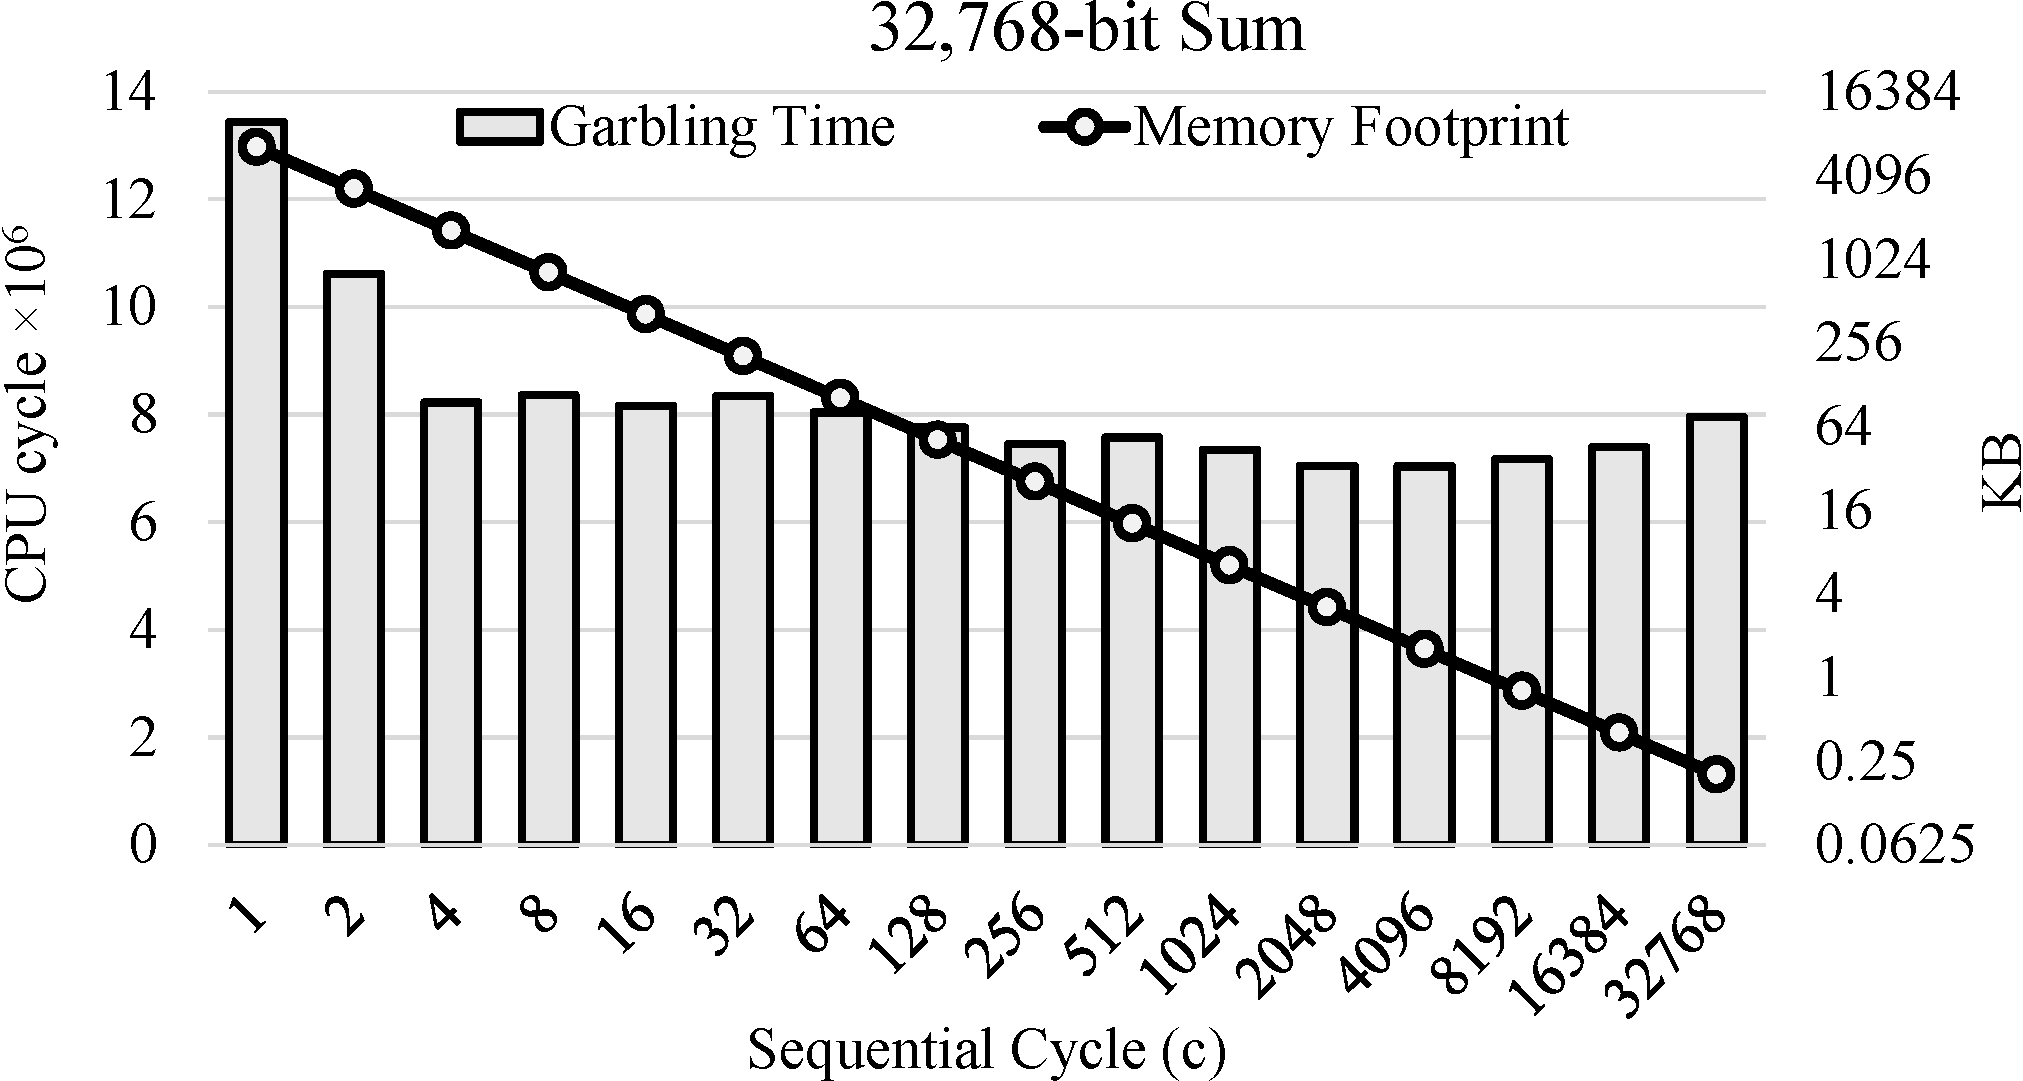
\includegraphics[width=0.7\textwidth]{CPU_Time-crop.pdf}
	\caption{Garbling $\numprint{32768}$-bit Sum function.
The CPU time in number of cycles and the approximate memory footprint in KBytes (y-axis) versus $c$ (x-axis) are shown.}
	\label{fig:cpu_time}
\end{figure}

\section{High Level Synthesis Tools}\label{sec:HLSeval}
The design automation community has been working on tools that work with higher-level languages and abstractions than HDL.
While a host of commercial and academic HLS tools are available \cite{tool:Vivado, tool:PandA, tool:MyHDL, Gupta2004}, we selected the Xilinx Vivado HLS for compiling C code to HDL which can then be synthesized using a conventional HDL synthesis tool.
The HLS engine in the Vivado suite is built upon the xPilot project \cite{Chapter:Zhang2008}.

\begin{table*}[t]
\centering
\caption{Comparison of performance of the circuits generated using C input to HLS and a direct Verilog input to the HDL synthesizer.}
\label{table:hls}
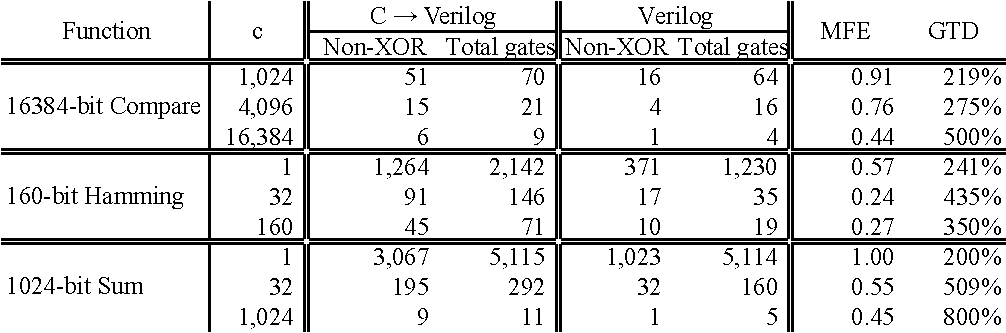
\includegraphics[scale=.9]{HLS-crop.pdf}
\end{table*}

Table \ref{table:hls} demonstrates a comparison between the performance of the circuits generated using C input to the HLS tool (C$\rightarrow$Verilog) and a direct Verilog input.
As can be seen from the table, the resulting memory footprint could increase by a factor between 1 and 4, while the number of garbled tables varies in a range of 3 to 9 times.
It is well known that writing the HDL level code which contains the time information and more detailed structural/behavioral description would yield much more efficient circuits than the code written in a higher level language.

\section{Evaluation of MIPS}\label{sec:mipsres}
We implement general purpose processor for PF-SFE using MIPS~I where one user provide function description in assembly and the other provides the data.
Support of sequential circuits in \sys{} enables us to use the MIPS circuit description in Plasma project \cite{rhoads2006plasma} without major modifications.
In the following, we provide the result of MIPS implementation and its memory footprint and communication load.
Lastly, we present implementation of Hamming distance with variable input length as a benchmark of private function application on MIPS.

\subsection{MIPS Implementation}
We used \sys{} to generate the netlist for the MIPS sequential circuit.
\tab{table:mipsres} shows the total number of gates and non-XOR gates for each module of the MIPS processor with $64\times32$bit DM and IM.
The sum of non-XORs for each module is $\numprint{14997}$.
However, when the modules are combined together to form the entire MIPS processor, the synthesizer optimizes the circuit such that the total number of non-XORs is reduced by $14.95\%$ to $\numprint{12755}$.
The memory footprint for storing tokens during garbling MIPS is approximately the size of two tokens times the total number of gates which is $2 \times 128 \times \numprint{31719}$bit $=991$~KB for token bit-width $k=128$.
The communication load between parties for invocation of one instruction (one sequential cycle) is approximately the size of three tokens times the number of non-XOR gates which is $3\times 128 \times \numprint{12755}$bit $=598$~KB with Row Reduction optimization.

\begin{table}[h]
\centering
\caption{Number of total gates and non-XOR gates in the MIPS implementation.
The global optimization of \sys{} reduces the overall number of gates compared to that of the sum of individual modules.}\label{table:mipsres}
\resizebox{0.4\textwidth}{!}{%
\begin{tabular}{l|rrl}
Modules             & Total gates & Non-XOR \\ \hline \hline
Controller          & 509                                                  & 470                                                \\
Bus                 & 603                                                  & 590                                                \\
ALU                 & 651                                                  & 346                                                \\
Shifter             & \numprint{1362}                                                 & \numprint{1092}                                               \\
Mult                & \numprint{2147}                                                 & \numprint{1792}                                               \\
Reg File            & \numprint{8880}                                                 & \numprint{3023}                                               \\
IM                  & \numprint{6048}                                                 & \numprint{2016}                                               \\
DM                  & \numprint{13779}                                                & \numprint{5423}                                               \\
PC                  & 309                                                  & 245                                                \\ \hline
Total               & \numprint{34288}                                                & \numprint{14997}                                              \\ \hline \hline
MIPS                & \numprint{31719}                                                & \numprint{12755}                                              \\ \hline \hline
\begin{tabular}[c]{@{}l@{}}Global \\optimization\end{tabular} & 7.49\%                                               & 14.95\%
\end{tabular}
}
\end{table}

\subsection{Benchmark: Hamming Distance}
We implemented the Hamming distance function as a proof-of-concept for our secure MIPS.
It counts the number of different elements in two arrays $A$ and $B$ with variable length $l$.
For the hand-optimized assembly code shown in \fig{figure:hamminassembly}, the function requires at most $7+9l$ sequential cycles (instructions) to evaluate.
Thus, based on \tab{table:mipsres}, this function requires overall $\numprint{12755}\times(7+9l)$ non-XOR gates.
It has only $16$ instructions and is stored in $16\times32$bit of the IM.
The function requires that $l$, $A$, and $B$ are stored in addresses $0$, $[2:l+1]$, and $[l+2:2l+1]$ of DM respectively.
It will store the Hamming distance of $A$ and $B$ in address $1$.

\begin{figure}
\lstinputlisting{Hamming.s}
\caption{Hamming distance assembly code.}\label{figure:hamminassembly}
\end{figure}

% !TEX root = 0_main.tex
\chapter{Related Work}\label{chap:related}
We classify related work into compilers for GCs (\sect{sect:GCCompiler}), libraries for GCs (\sect{sect:GCLibs}), GC implementations with hardware accelerators (\sect{sect:HWaccel}), and GC implementations on mobile devices (\sect{sect:mobile}).

\section{Compiler for Garbled Circuits}\label{sec:GCCompiler}
The following tools compile high level function descriptions into a Boolean circuit which can be used in GC.
The first realization of GCs was Fairplay \cite{malkhi2004fairplay} which provides a custom high level procedural language called SFDL (Secure Function Definition Language) that is compiled into a circuit description language, SHDL (Secure Hardware Description Language).
Another compiler is TASTY \cite{HKSSW10} which allows to combine garbled circuits and homomorphic encryption.
The compiler of \cite{kreuter2012billion} for the first time showed scalability to circuits consisting of billions of gates, e.g., a 4095x4095-bit edit distance circuit with almost 6 Billion gates.
The compiler of \cite{franz2014cbmc} allows to use a subset of ANSI C as input language.

To reduce the memory overhead for storing large circuits and hence increase scalability, PCF \cite{kreuter2013pcf} introduced loops that, if given manually in the high level language, are kept until the GC evaluation.
In contrast to PCF, \sys{} allows to infer loops automatically and also allows to optimize across multiple sub-circuits.

\section{Libraries for Garbled Circuits}\label{sec:GCLibs}
Instead of compiling circuits, FastGC \cite{huang2011faster} proposed to use a library-based approach where circuits can be programmed and easily integrated into high-level applications.
Another GC library is VMCRYPT \cite{malka2011vmcrypt} that allows to dynamically construct and deconstruct sub-circuits.
FastGC was extended in \cite{HS13} to re-use the same sub-circuits.
Another library for secure computation is ABY that allows the efficient combination of multiple secure computation approaches \cite{DSZ15}.

In all these library-based approaches the circuits and their decomposition into sub-circuits has to be specified manually by the programmer, whereas we provide an automated approach.

\section{GC Implementations with Hardware Accelerators}\label{sec:HWaccel}
The following works provide better performance by implementing garbled circuits in hardware, on GPUs, or using AES-NI available in recent CPUs.
These works can benefit from the compact representation generated by \sys.

J\"arvinen et al., \cite{jarvinen2010garbled} proposed a generic hardware architecture for GC.
They realized two FPGA-based prototypes: a system-on-a-programmable-chip with access to a hardware crypto accelerator targeting smartcards and smartphones, and a stand-alone hardware implementation targeting ASICs.

Recently, several accelerations of GCs using GPUs have been proposed.
Husted et al., implemented Yao's GC by using optimizations such as Free XOR, pipelining, and OT extension \cite{husted2013gpu}.
Pu et al., realized dynamic programming based on GC to solve the Edit-Distance (ED) and the Smith-Waterman (SW) problems \cite{pu2013computing}.
They also used the same optimizations as \cite{husted2013gpu} along with permute-and-encrypt, efficient lookup-table design, and compact circuits \cite{pu2013computing}.
Frederiksen et al., implemented a secure computation protocol with security against malicious adversaries based on cut-and-choose of Yao's garbled circuit and an efficient OT extension for two-party computation on GPUs \cite{frederiksen2013fast}.

Bellare et al., propose JustGarble in which they use fixed-key AES for circuit-garbling \cite{bellare2013efficient}.
They show their implementation using AES-NI can efficiently garble and execute a circuit far faster than any prior report.

\section{GC Implementations on Mobile Devices}\label{sec:mobile}
Our approach for generating compact circuit representations is also beneficial when performing secure computation on resource constrained devices such as mobile devices which have a limited amount of main memory.
Secure computation on mobile devices using garbled circuits was proposed in \cite{HCE11}.
Also the protocol described in \cite{DSZ14}, which uses a smartcard installed in the mobile device, can benefit from our more compact circuit representation.
In \cite{CMTB13, CLT14} the mobiles no longer need to process circuits any more as GC generation and evaluation is outsourced to cloud servers.

% !TEX root = 0_main.tex
\chapter{Conclusion and Future Directions}\label{chap:conc}
We present \sys{}, an automated tool that can generate highly compact and scalable circuits for Yao's garbled circuit (GC) protocol.
We are the first to define the circuit generation for GC as a sequential synthesis problem, and to leverage the powerful and established HDL synthesis techniques with our custom-libraries and objectives.
We improve the results of one of the best automatic tools for GC generation, PCF \cite{kreuter2013pcf}, by several orders of magnitude: for instance \sys{} compacts the $\numprint{1024}$-bit multiplication by $\numprint{2504}$ times, while decreasing the number of non-XOR gates by 80\%; we compress the $\numprint{16000}$-bit Hamming distance by a factor of $\numprint{7345}$ times and with 47\% less non-XOR gates.
Further, \sys{} is able to implement functions that have never been reported before, such as SHA-3.
We perform extensive benchmarking with both commercial and open source hardware synthesis tools and compare the results.
Our approach strongly improves the existing results towards practical secure computation with many exciting applications.
For instance, \sys{} is an enabling technology for performing GC operations on mobile platforms, which is prohibitively expensive using the prior techniques.
Moreover, we introduce a scalable secure processor for private function evaluation (PF-SFE).
The processor is based on the MIPS architecture and the private function can be compiled using ubiquitous tool, e.g., gcc.
In future work we will investigate the possibility of connecting Oblivious RAM (ORAM) to our secure processor to benefit from its lower amortized complexity for memory access.
We are also working on interfacing \sys{} with other GC schemes, e.g., the recently proposed Half Gates method \cite{zahur2014two}.

\appendices
% !TEX root = 0_main.tex
\chapter*{Open Source Logic Synthesis Tools}\label{app:seqos}
\sys{} offers a generic methodology for generating GC that is transparent to the underlying logic synthesis tool.
To show this point, we demonstrate an implementation of \sys{} using the Yosys \cite{tool:Yosys} and ABC \cite{tool:ABC} logic synthesis tool chain for circuit generation.
Both of these tools are open-source and available online.
We compare the performance of the commercial HDL synthesis tool, i.e., Synopsys DC, with this open-source synthesis tool chain.
ABC is an academic package developed at the University of California Berkeley.
Yosys is an HDL-based synthesis tool which calls ABC for its technology mapping.
The HDL inputs for describing both sequential and combinational circuits are written in the Verilog programming language.

We compare the performance of these open-source tools to the commercially available Synopsys DC.
The results are presented in \tab{table:abc}.
For comparison purposes, we compute $\mathit{GTD}$ and $\mathit{MFE}$ using the netlists generated by Synopsys DC as reference.
For most of the benchmarks $\mathit{GTD}$s are either very small or zero which implies that the number of non-XOR gates in circuits generated by Yosys and by Synopsys DC are almost similar.
In terms of memory footprint, different tools perform better for different benchmark functions.
These results shows that \sys{} is transparent to the underlying logic synthesis tool as long as the tool is up to date with respect to the known methods for logic minimization and mapping.
Since the logic synthesis tools perform a series of optimizations, they may use different (heuristic) algorithms for some of their internal steps which could lead to slightly different results.
A user can choose between different synthesis tools based on their performance and availability.

\begin{table}[h]
\caption{Comparison of circuit generation performance between the commercial Synopsys DC and Yosys+ABC open source logic synthesizer.}
\label{table:abc}
\centering
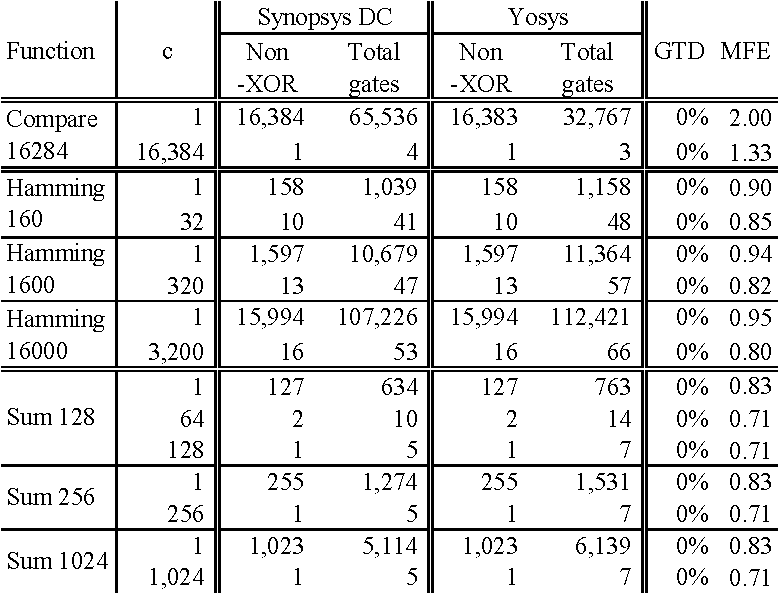
\includegraphics[scale=.9]{abc-crop.pdf}
\end{table}


\bibliographystyle{ieeetr}
\bibliography{main_bib}
\end{document}
